%%=========================================
\section[Eksperimenter \& Resultater]{Eksperimenter \& Resultater}
%%=========================================
\subsection{Evalueringsstrategier}
{\color{red}Hvordan kan eksperimentene evalueres?}

\subsection{Utførelse eksperimenter}
{\color{red}Hvordan ble eksperimentet utført?}

\subsubsection*{Gestegjenkjennelse gjennom fotodioder}
{\color{red}Hvordan ble eksperimentet utført?}
{\color{red}Dette avsnittet må kanskje skrives ut mye mer for å forklare stegvis alt som er gjort?}
For å trene disse klassifikatorene kreves data. For å koble Arduinoen opp til sensoren fulgte jeg SparkFun's oppkoblingsguide\footnote{https://learn.sparkfun.com/tutorials/apds-9960-rgb-and-gesture-sensor-hookup-guide?\_ga\=1.23518458.1114877585.1417681856}. Etter at Arduinoen er koblet til sensoren og til datamaskinen ved en usb-kabel kan man laste opp koden som trengs for å drive sensoren. Biblioteket SparkFun tilbyr ble tilpasset til å ikke selv forstå sensordataene, men i stedet dytte dem videre til datamaskinen. Når Python-scriptet{\color{red} ref process-data.py} kjøres på datamaskinen åpnes tilkoblingen til å lytte på den riktige serielle porten. Porten åpnes i noen sekunder og ber om at en gest utføres. Jeg gjennomførte 50 utførelser av hver av de 10 gestene\ref{fig:gester}, for totalt 500 datapunkter. Dataene fra hver gest ble lagret i individuelle filer i kommaseparert format. Med dataene for hver gest lagret i forskjellige filer kan disse kombineres slik man ønsker for å trene systemet til å skille mellom 2,3, eller opp til 10 gester. 

Python-scriptet {\color{red} ref learning.py} utfører maskinlæringen. Dataene blir lastet inn fra de aktuelle csv-filene og de aktuelle klassene opprettes. Man splitter så dataene i et treningssett og et testsett. Splittingen var 75\% til trening og 25\% til testing. Dette er et viktig steg i prosessen for å ikke spesialisere modellen til dataene. Dersom man trener på hele datasettet og tester på det samme settet er det en sjanse for at man har tilpasset modellen for mye til datasettet og ikke funnet den underliggende, generelle modellen. Hver modell blir trent og testet 100 ganger med et tilfeldig utgangspunkt hver gang, og sluttresultatet er et gjennomsnitt av disse.

\subsubsection{Multimodal interaksjon gjennom tale og gester}
{\color{red}Hvordan ble eksperimentet utført?}

\subsubsection{Kombinasjoner}
{\color{red}Hvordan ble eksperimentet utført?}

\subsubsection{Kontekstdrevet brukergrensesnitt}
{\color{red}Hvordan ble eksperimentet utført?}





\subsection{Resultater}
\subsubsection{Gestegjenkjennelse gjennom fotodioder}
{\color{red}Hva var resultatet av eksperimentet?}
\label{ch:2.resultater}
\begin{table}[h!]
\centering
\begin{tabular}{|| c c c ||}
\hline
\% Korrekt klassifisering & Algoritme & Antall treningseksempler\\ [0.5ex] 
 \hline\hline
 96,0 & SVM m/libsvm & 500 \\ 
 \hline
 95,8 & SVM m/liblinear & 500 \\
 \hline
 94,048 & Logistisk regresjon & 500 \\ [1ex]
 \hline
\end{tabular}
\caption{Gjennomsnittsresultater for klassifisering der modellene er trent og testet 100 ganger med tilfeldige utgangspunkt.}
\label{table:results}
\end{table}

\begin{figure}[h!]
\centering
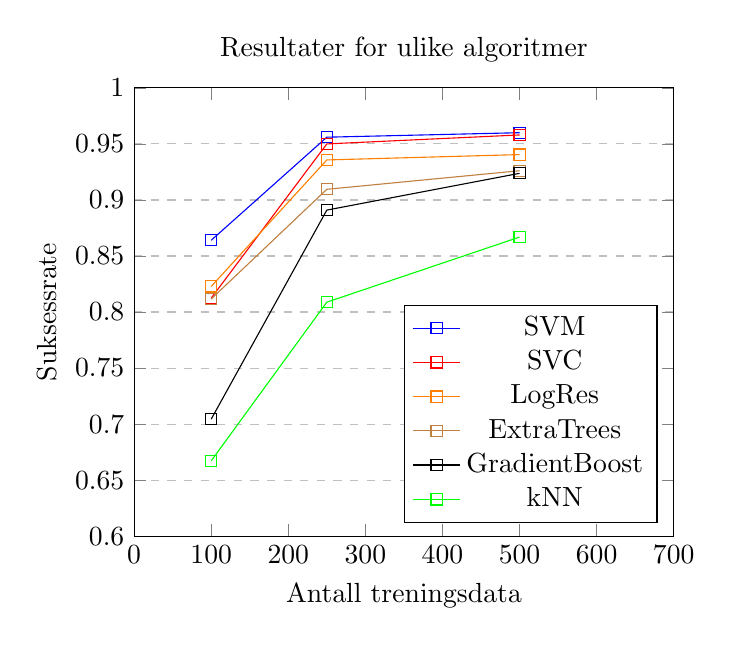
\begin{tikzpicture}
\begin{axis}[
    title={Resultater for ulike algoritmer},
    xlabel={Antall treningsdata},
    ylabel={Suksessrate},
    xmin=0, xmax=700,
    ymin=0.6, ymax=1.0,
    xtick={0,100,200,300,400,500,600,700},
    ytick={0.6,0.65,0.7,0.75,0.8,0.85,0.9,0.95,1.0},
    legend pos=south east,
    ymajorgrids=true,
    grid style=dashed,
]
\addplot[
    color=blue,
    mark=square,
    ]
    coordinates {
    (100,0.864)(250,0.956)(500,0.96)
    };
\addplot[
    color=red,
    mark=square,
    ]
    coordinates {
    (100,0.8124)(250,0.95)(500,0.958)
    };
\addplot[
    color=orange,
    mark=square,
    ]
    coordinates {
    (100,0.8228)(250,0.9357)(500,0.94048)
    };
\addplot[
    color=brown,
    mark=square,
    ]
    coordinates {
    (100,0.8116)(250,0.9095)(500,0.92608)
    };
\addplot[
    color=black,
    mark=square,
    ]
    coordinates {
    (100,0.7044)(250,0.89095)(500,0.92376)
    };
\addplot[
    color=green,
    mark=square,
    ]
    coordinates {
    (100,0.6672)(250,0.8088)(500,0.86688)
    };
    
    \legend{SVM,SVC,LogRes,ExtraTrees,GradientBoost,kNN}
\end{axis}
\end{tikzpicture}
\label{figure:resultsgraf}
\caption{Resultatsutvikling for et utvalg algoritmer.}
\end{figure}

Både logistisk regresjon og støttevektormaskin ga svært lovende resultater, som vist i tabell \ref{table:results}. 96\% er en meget høy suksessrate og viser hvor godt enkle, lineære modeller kan skille på denne typen data. Det ble så interessant å spørre seg om dette resultatet kunne blitt enda høyere. Jeg ønsket ikke å bruke mer tid på å lage flere treningseksempler, så i stedet utførte jeg treningen på nytt med færre treningseksempler, i håp om å kunne se en utviklingstrend. Det samme eksperimentet ble utført med en femtedel og halvparten av dataene for å danne et bilde av sammenhengen mellom forbedring i suksessrate og antall treningseksempler. Figur \ref{figure:resultsgraf} viser resultatene for 100, 250 og 500 treningseksempler. Ettersom biblioteket jeg benyttet for å implementere algoritmene tilbyr en rekke andre algoritmer forsøkte jeg noen andre tilnærminger enn lineære modeller og inkluderte dem også.

I figur \ref{figure:resultsgraf} kan vi se at SVM-ene er i nærheten av 95\% allerede etter 250 treningseksempler og at de kun øker minimalt med 250 ekstra tilfeller. Dette tyder på at det trengs et stort antall ekstra treningseksempler for at algoritmene skal krype betydelig nærmere 100\%. De mer kompliserte algoritmene ExtraTrees og GradientBoost benytter seg av flere algoritmer under panelet og kombinerer disse. Det kan se ut som om spesielt GradientBoost kan fortsette å øke suksessraten betydelig med mer trening, men det er tvilsomt om den noen gang passerer SVM. Til sist nevnes k-nærmeste nabo (kNN), som begynner svakest av de utprøvde algoritmene, men fremdeles har en sterk vekst mellom 250 og 500 tilfeller. Det hadde vært interessant å se utviklingen videre for denne enkle algoritmen.

Dette prosjektet har argumentert for at gester kan være en aktuell interaksjonsform i hjemmet, spesielt som en erstatning til store knappepaneler og desentralisert styringskontroll. Det har også vist at maskinlæring kan benyttes for å gi enkle sensorer en svært god forståelse av gester. Med en suksessrate på over 95\% i klassifiseringen av 10 ulike gester er denne teknikken svært interessant. Og med en suksessrate på over 85\% allerede etter kun 10 treningseksempler på hver gest, kan man forestille seg at brukere selv kan sette av 10 minutter til å trene et helt nytt og utrent system til å forstå sine egne gester. I et produkt kunne det vært aktuelt å tilby online-læring gjennom systemets levetid. Man kan med andre ord la systemet lære etter hvert som brukeren benytter systemet. Dette vil nødvendigvis kreve at brukeren har en mulighet til å gi tilbakemelding på når systemet gjettet riktig gest og når det gjettet feil.

\subsubsection{Multimodal interaksjon gjennom tale og gester}
{\color{red}Hva var resultatet av eksperimentet?}
Dette kapittelet har følgende bidrag:
\begin{itemize}
\item Argumenterer for at kombinasjonen av enkle gester og talekommandoer er en effektiv måte å interagere med det smarte hjemmet på {\color{red} fwd ref}.
\item Viser at talegjenkjenning over en begrenset mengde ord dekker funksjonaliteten vi ønsker å tilby gjennom tale og at det finnes åpne og tilgjengelige løsninger for å løse dette problemet.{\color{red} fwd ref}.
\item En implementasjon som håndterer multimodal input fra gestesensor og mikrofon. Denne benyttes for å simulerer bruken i et smart hjem ved å vise en dynamisk grafisk representasjon av inputdataene. Forskjellige anvendelser blir utforsket. {\color{red} fwd ref}.
\end{itemize}

\subsubsection{Kombinasjoner}
{\color{red}Hva var resultatet av eksperimentet?}

\subsubsection{Kontekstdrevet brukergrensesnitt}
{\color{red}Hva var resultatet av eksperimentet?}
